% D.35 斜坡：坡比 1:√3（即 tan α = 1/√3 → α=30°），坡面长 20 m
\documentclass[tikz,border=4pt]{standalone}
\usepackage{ctex}
\usepackage{amsmath}
\usetikzlibrary{calc}
\begin{document}
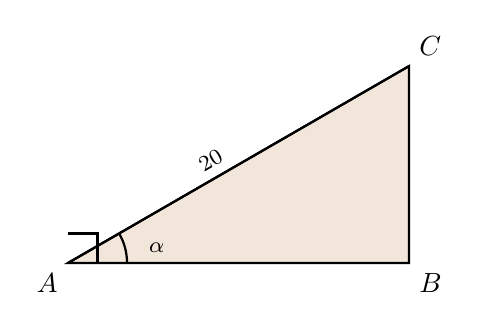
\begin{tikzpicture}[scale=0.25, thick]
  \coordinate (A) at (0, 0);
  \coordinate (C) at ({20*cos(30)}, {20*sin(30)});
  \coordinate (B) at ({20*cos(30)}, 0);

  \fill[brown!20] (A) -- (B) -- (C) -- cycle;
  \draw (A) -- (B) -- (C) -- cycle;
  \draw (A) -- (C);

  \draw (1.5, 0) -- (1.5, 1.5) -- (0, 1.5);

  \draw (3, 0) arc[start angle=0, end angle=30, radius=3];
  \node at (4.5, 0.8) {\footnotesize $\alpha$};

  \node[below left]  at (A) {$A$};
  \node[below right] at (B) {$B$};
  \node[above right] at (C) {$C$};
  \node[above left, rotate=30] at ($(A)!0.5!(C)$) {\footnotesize $20$};
\end{tikzpicture}
\end{document}
